\documentclass{article} % For LaTeX2e
\usepackage{nips14submit_e,times}
\usepackage{hyperref}
\usepackage{url}
\usepackage{amsmath}
\usepackage{amssymb}
\usepackage{bbm}
\usepackage{tikz}
\usepackage{tikz-qtree}
\usepackage[sort&compress]{natbib}
\usepackage{natbibspacing}
\usepackage{multirow}

\usetikzlibrary{arrows}
\usetikzlibrary{shapes, trees}

\bibliographystyle{unsrt}

\DeclareMathOperator*{\argmax}{argmax}
\DeclareMathOperator*{\argmin}{argmin}

\newcommand{\unorderedS}{\mathcal{S}^{\mathrm{u}}}
\newcommand{\orderedS}{\mathcal{S}^{\mathrm{o}}}
\newcommand{\ourmethod}{NCL}

\newcommand{\bmcomment}[1]{\textcolor{blue}{\textsc{\textbf{[#1 --bm]}}}}
\newcommand{\nascomment}[1]{\textcolor{red}{\textsc{\textbf{[#1 --nas]}}}}
%\documentstyle[nips14submit_09,times,art10]{article} % For LaTeX 2.09


\title{Learning Not to Try Too Hard}

\author{
Bill McDowell\thanks{Alternative email: \texttt{forkunited@gmail.com}} \\
School of Computer Science\\
Carnegie Mellon University\\
Pittsburgh, PA 15213 \\
\texttt{wmcdowel@cs.cmu.edu} \\
\And
Noah A.~Smith \\
School of Computer Science\\
Carnegie Mellon University\\
Pittsburgh, PA 15213 \\
\texttt{nasmith@cs.cmu.edu} \\
}

% The \author macro works with any number of authors. There are two commands
% used to separate the names and addresses of multiple authors: \And and \AND.
%
% Using \And between authors leaves it to \LaTeX{} to determine where to break
% the lines. Using \AND forces a linebreak at that point. So, if \LaTeX{}
% puts 3 of 4 authors names on the first line, and the last on the second
% line, try using \AND instead of \And before the third author name.

\newcommand{\fix}{\marginpar{FIX}}
\newcommand{\new}{\marginpar{NEW}}

\nipsfinalcopy % Uncomment for camera-ready version

\begin{document}

\maketitle

%\bmcomment{It seems like a lot of other papers refer to 'cost' as 'loss'... 
%Is there somewhere where people call it 'cost' like we are?}
%\nascomment{will address this}

%\begin{abstract}
%\nascomment{do last}
%\end{abstract}

\section{Introduction}

Discriminative learning algorithms are often motivated by their
ability to trade off among different kinds of prediction mistakes with
different costs.  The cost of a mistake is usually taken to be fully
defined by the task, i.e., human system designers are trusted to
encode this knowledge prior to learning.  Information about the
inherent ease of avoiding some errors vs.~others is generally not
taken into account.   Closely related to this, and critically
important in domains where the data is constructed by humans, is the
problem that the outputs in the training data may be unreliable.  For
example, if training data is produced by asking humans to label
instances, and two labels are insufficiently well defined for human
labelers to distinguish them,
then a learner might be forgiven for conflating them.

We consider situations where human intuition about relative costs of
different errors is insufficient.  In a margin-based linear modeling
framework, we propose a method for incorporating \textbf{learning of
  the cost function} alongside learning of the model.  Our approach
introduces explicit estimates of the ``ease'' of avoiding each type of
error
(for a particular model family).   For error types that are ``just too
hard,'' our model is offered the possibility of giving up in favor of
making other, less challenging predictions more accurately



%\bmcomment{Might want to give some motivating examples? Not sure if that's
%necessary or not. One example of multiclass domain, and one example where
% cost functions are used in structured domains} 

% \bmcomment{Mention examples of measures of 'difficulty'? Cite.}

\bmcomment{Modify this.}
Our experiments with text classification show  scenarios where the method achieves
performance improvements over a strong baseline.


\section{Background and Notation}

In a prediction problem, let $\mathcal{X}$ denote the input space,
$\mathcal{Y}$ denote the output space, and assume $N$ training
instances $\{(x_1, y_1), \ldots, (x_N, y_N)\}$.  We assume a linear
model and prediction function:
\begin{equation}
\hat{y} = \argmax_{y \in \mathcal{Y}} \left(f(x, y;\mathbf{w}) \triangleq \mathbf{w}^\top \mathbf{g}(x, y) \right)
\end{equation}
where $\mathbf{w} \in \mathbb{R}^D$ are the parameters to be learned
and $\mathbf{g} : \mathcal{X} \times \mathcal{Y} \rightarrow
\mathbb{R}^D$ is the feature vector function.  We will let
$\mathcal{M} =\{f(\cdot,\cdot;\mathbf{w}) \mid \mathbf{w} \in
\mathbb{R}^D\}$ denote the model family under consideration, given a
fixed choice of $\mathbf{g}$.

Our approach, which assumes $\mathcal{Y}$ is categorical, is based on
the soft margin formulation of multiclass support vector machines
\citep{vapnik1998statistical,crammer2002algorithmic,weston1998multi}.
Tsochantaridis et al.~\citep{tsochantaridis2004support} and Taskar et
al.~\citep{koller2003max} generalized this framework to allow for
differences in costs between different kinds of mistakes, as found
when $\mathcal{Y}$ is structured.  Let the cost function
$\Delta:\mathcal{Y}\times\mathcal{Y}\rightarrow\mathbb{R}$  be such
that $\Delta(y, y')$ is the cost of predicting $y$ when the correct
label is $y'$.  We use the ``margin rescaling'' variant the multiclass SVM:
\begin{align}
 \min_{\boldsymbol{\xi}\geq 0, \mathbf{w}}
\frac{\lambda}{2}\|\mathbf{w}\|_2^2+\frac{1}{m}\sum_{i=1}^N\xi_i 
 \text{\ \ \ s.t.\ \ \ } \forall i,  \forall y \in \mathcal{Y} \setminus
 \{y_i\},  f(x_i, y_i; \mathbf{w}) - f(x, y, \mathbf{w}) \geq
 \Delta(y, y_i) - \xi_i \label{marginRescaling}
\end{align}
This objective seeks $\mathbf{w}$ that minimizes misclassifications while
maximizing the margin between correct and incorrect instances.
Further, the more incorrect an $(x,y)$ pair is, the greater the margin
should be.  This problem is often transformed into an unconstrained
one corresponding to direct minimization of the regularized average
hinge loss:
\begin{equation}
\label{svmObjective}
\min_{\mathbf{w}} \frac{\lambda}{2}\|\mathbf{w}\|_2^2 +
\sum_{i=1}^N  -f(x_i, y_i; \mathbf{w}) + \max_{y \in \mathcal{Y}}
  f(x_i, y; \mathbf{w}) + \Delta(y, y_i)
\end{equation}

We introduce some notation for errors.
We let $\mathcal{S} \subseteq 2^{\mathcal{Y}\times\mathcal{Y}}$ be a
collection of prediction error classes that 
exhausts $\mathcal{Y}^2$ (i.e., $\bigcup_{S \in
  \mathcal{S}} S = \mathcal{Y}^2$); the error 
  classes need not be
mutually exclusive.  We let $e_{S} \in \mathbb{R}$ denote an estimate
of the ``ease'' with which a learner searching in $\mathcal{M}$ 
can successfully avoid errors in class $S$.  Then we let:
\begin{equation}
\Delta(y, y') = \sum_{S \in \mathcal{S}: (y, y') \in S} e_S =
\mathbf{e}^\top \mathbf{s}(y, y')
\end{equation}
where $\mathbf{e}$ is a vector of the $e_S$ and $\mathbf{s}$ is a
binary vector of length $\mathcal{S}$ indicating which error class(es)
each possible confusion in $\mathcal{Y}\times\mathcal{Y}$ belongs to.

In this paper, we consider two prediction error classes, corresponding
to unordered and ordered pairs of outputs.  We denote them
$\unorderedS$ and $\orderedS$, respectively.  

% There are many possible choices for prediction classes $\mathcal{S}$, but
% in this paper, we focus on the following two:

% \begin{equation}
% \begin{split}
% & \mathcal{S}_{[\mathcal{Y}]^2} = \{ S_{\{\mathbf{y},\mathbf{y}'\}} | \mathbf{y},\mathbf{y}'\in\mathcal{Y}\} \\
% \text{ where } & S_{\{\mathbf{y},\mathbf{y}'\}}=
% \{ (\mathbf{y}_1, \mathbf{y}_2) | (\mathbf{y}_1=\mathbf{y}\wedge \mathbf{y}_2=\mathbf{y}')\vee(\mathbf{y}_1=\mathbf{y}'\wedge \mathbf{y}_2=\mathbf{y}) \} \\
% \end{split}
% \end{equation}

% \begin{equation}
% \mathcal{S}_{\mathcal{Y}^2} = \{ S_{(\mathbf{y},\mathbf{y}')} | \mathbf{y},\mathbf{y}'\in\mathcal{Y}\}\text{ where }S_{(\mathbf{y},\mathbf{y}')}=\{ (\mathbf{y},\mathbf{y}') \} \\
% \end{equation}

% $\mathcal{S}_{[\mathcal{Y}]^2}$ contains a prediction class for every
% unordered pair of labels, and $\mathcal{S}_{\mathcal{Y}^2}$ contains
% a prediction class for every ordered pair.  We might choose 
% $\mathcal{S}_{[\mathcal{Y}]^2}$ when factoring the cost function if
% we believe it is equally easy to resolve misclassifications of 
% $\mathbf{y}$ as $\mathbf{y}'$ and misclassifications of $\mathbf{y}'$
% as $\mathbf{y}$.  Otherwise, if we suspect these two incorrect 
% prediction types to differ in easiness, then we might choose 
% $\mathcal{S}_{\mathcal{Y}^2}$.

\section{Cost Learning Model}
\label{costLearningModel}


Previous work assumes $\Delta$ follows intuitively from the prediction
task.  For example, in natural language dependency parsing, the number
of words attached to the wrong parent (Hamming distance for the parse
tree) is a sensible choice.  
We propose to parameterize $\Delta$ and
learn its parameters jointly with $\mathbf{w}$.  This learned cost
function should encode distances between outputs from the perspective
of the ease with which a model in the family $\mathcal{M}$
can distinguish between them.
This joint learning setup is expected to be particularly useful when
some classes of errors are difficult or impossible for a model in the
class to resolve, due to unreliable annotations or an insufficient
choice of features $\mathbf{g}$.


\subsection{Ease}
\label{sec:ease}
We desire a model that estimates prediction ease $\mathbf{e}$ while
estimating
predictive model parameters $\mathbf{w}$. 
We have used the term ``ease''
with respect to an arbitrary model in the family $\mathcal{M}$, but it
is more sensible to consider the particular model we seek to
estimate.  We propose that, for error class $S$ and a model with
parameters $\mathbf{w}$, ease $e_S$ should be inversely related to the
number of
of margin violations involving $S$ that $f(\cdot, \cdot; \mathbf{w})$ makes in the
training data assuming that $\argmax$ always gives a 
single label, breaking ties arbitrarily:

\begin{equation}
v_S (\mathbf{w}, \mathbf{e}) \triangleq \left|\left\{ i  \in \{1,\ldots, D\} \mid \left(y_i, \textstyle \argmax_{y \in \mathcal{Y}} f(x_i, y ; \mathbf{w}) +
\mathbf{e}^\top \mathbf{s}(y, y_i)\right) \in S\right\}\right| \label{eq:set}
\end{equation}

The intuition is that, when this set is large, it is because it is not easy for the
model to shrink.  Of course, we should also take into account 
that the distribution of the data may make some errors more frequent,
inflating the size of the set in Eq.~\ref{eq:set} even if $S$ is ``easy.''
Further,  \emph{infrequently} observed labels are generally
expected to be harder to predict.  Yet for an $S$ that includes errors on
a  rarely occurring class, the set in Eq.~\ref{eq:set} will
necessarily be small, regardless of how easy it is.
We therefore propose the following condition for $e_S$:
\begin{equation}
e_S = \max\left( 0, 1 - \frac{v_S(\mathbf{w}, \mathbf{e}) }{n_S}\right) \label{e-condition}
\end{equation}
where $n_S$ is a fixed, \emph{a priori} upper bound on the count of
$S$ errors, $v_S$.   This
has the desirable property that  if $v_S \ge n_S$,  i.e., $S$ is too
difficult to shrink, then ease $e_S$ goes to zero and the model is
allowed to give up on $S$.  It also keeps $e_S \in [0,1]$, 
ensuring interpretability of the ease relative to the
maximum possible value of $e_S=1$.

% The size of $S_{\mathcal{M},\mathbf{g},D}$ is the number of
% training examples with margin violations in class $S$. If
% the size of this set is large, we might infer that the
% model has trouble shrinking it, and so it's not 'easy'.  This 
% might lead us to conclude that $S_{\mathcal{M},\mathbf{g},D}$ 
% tends to shrink with 'easiness'.  However,
% for many data sets and choices of $\mathcal{S}$, the size 
% of each $S_{\mathcal{M},\mathbf{g},D}$ can be inherently
% biased by the data independently of 'easiness'.  For example, 
% for $S_{\{\mathbf{y},\mathbf{y}'\}}\in\mathcal{S}_{[\mathcal{Y}]^2}$, 
% the size of $S_{\{\mathbf{y},\mathbf{y}'\},\mathcal{M},\mathbf{g},D}$ 
% is biased by the number of examples in the training data which have 
% output labels $\mathbf{y}$ and $\mathbf{y}'$--if there are few 
% training examples of labels 
% $\mathbf{y},\mathbf{y}'\in\mathcal{Y}$, then the size of 
% $S_{\{\mathbf{y}, \mathbf{y}'\},\mathcal{M},\mathbf{g},D}$ 
% will necessarily be small relative to other prediction classes.
% Furthermore, we expect 
% output labels which occur infrequently in the training data to 
% be more difficult for the model to predict correctly, so this
% will lead to the size of 
% $S_{\{\mathbf{y},\mathbf{y}'\},\mathcal{M},\mathbf{g},D}$ 
% increasing with the 'easiness' of 
% $S_{\{\mathbf{y},\mathbf{y}'\}}$ which is opposite the 
% conclusion that that we draw if we think of the size of 
% $S_{\{\mathbf{y},\mathbf{y}'\},\mathcal{M},\mathbf{g},D}$ as
% increasing due to the model's difficulty in shrinking it.  In general, 
% this suggests that if we want the size of $S_{\mathcal{M},\mathbf{g},D}$
% to vary with easiness, we need to normalize it to account for 
% properties of the training data that introduce irrelevant
% biases.  

\subsection{Objective}

Our approach is a modification to the SVM objective in
Eq.~\ref{svmObjective}; it is a joint optimization of $\mathbf{w}$ and $\mathbf{e}$:
\begin{equation}
\label{costObjective}
\min_{\mathbf{e}\geq 0,\mathbf{w}} \frac{\lambda}{2}\|\mathbf{w}\|_2^2
+ \frac{1}{2} \|\mathbf{e}\|_{\mathbf{n}}^2 - \mathbf{e}^\top
\mathbf{n} + \sum_{i=1}^N -f(x_i,y_i; \mathbf{w})  + \max_{y \in
  \mathcal{Y}} f(x_i,y ; \mathbf{w}) + \mathbf{e}^\top \mathbf{s}(y, y_i)
\end{equation}
where $\mathbf{n}$ is the vector of upper bounds on prediction error
frequencies and $\|\mathbf{e}\|_{\mathbf{n}}^2 = \sum_{S \in
  \mathcal{S}} n_Se_S^2$.  The changes amount to (1) including
$\mathbf{e}$ as a free variable and (2) regularizing it with a quadratic
penalty (second term in Eq.~\ref{costObjective}) and a linear penalty
(third term in Eq.~\ref{costObjective}).  The linear penalty selects
which $e_S$ should be nonzero---equivalently, are not impossibly
difficult. Setting $e_S=0$ amounts to giving up on $S$
errors.\footnote{The meaning of 'giving up' is unclear.  It seems
that setting $e_S=0$ actually amounts to giving up on margin maximization,
but not error minimization with respect to $S$, but we don't work 
this out in detail.\bmcomment{Noah, do you understand
this differently?}}

Most importantly, Eq.~\ref{costObjective} is minimized at $\mathbf{e}$ 
that matches Eq.~\ref{e-condition}.  To see this, we can find the 
subdifferential $\partial C$ of the function $C$ minimized in
Eq.~\ref{costObjective}, and consider the optimized ease values 
$\mathbf{e}^*$
for which $\mathbf{0}\in \partial C(\mathbf{w}^*,\mathbf{e}^*)$.  
$\partial C$ is given by:

\begin{equation}
\label{subdifferential}
\begin{split}
\partial C(\mathbf{w},\mathbf{e}) = & \frac{\lambda}{2}\nabla (\|\mathbf{w}\|_2^2)
+\frac{1}{2}\nabla (\|\mathbf{e}\|^2_{\mathbf{n}})-\nabla (\mathbf{e}^\top \mathbf{n})
+ \\ 
& \sum_{i=1}^N -\nabla (f(x_i,y_i; \mathbf{w}))+ 
\mathbf{Co}(\nabla F^{\Delta}_{\max}(x_i,y_i;\mathbf{w},\mathbf{e}))
\end{split}
\end{equation}

Where addition, subtraction, and $\nabla$ are overloaded to perform sums,
subtractions, and gradients over sets, 
$\mathbf{Co}(\cdot)$ gives the convex hull of a
set, and $F^{\Delta}_{\max}$ is defined as:

\begin{equation}
\label{FmaxDef}
F^{\Delta}_{\max}(x,y;\mathbf{w},\mathbf{e}) = 
\{ f(x, \hat{y} ; \mathbf{w}) +
\mathbf{e}^\top \mathbf{s}(y, \hat{y})
| \hat{y}\in\argmax_{y' \in \mathcal{Y}} f(x, y' ; \mathbf{w}) +
\mathbf{e}^\top \mathbf{s}(y, y') \}
\end{equation}

We are only interested in the value of $\mathbf{e}$, so
we can consider Eq.~\ref{subdifferential} reduced to 
a simpler subdifferential 
with respect to a single component $e_S$ of $\mathbf{e}$:

\begin{equation}
\label{eSubdifferential}
\partial_{e_S} C(\mathbf{w},\mathbf{e}) = 
n_S e_S -n_S+
\sum_{i=1}^N 
\mathbf{Co}(\frac{\partial 
F^{\Delta}_{\max}(x_i,y_i;\mathbf{w},\mathbf{e})}{\partial e_S})
\end{equation}

Given that $\mathbf{0}\in \partial C(\mathbf{w}^*,\mathbf{e}^*)$,
Eq~\ref{eSubdifferential} leads to:

\begin{equation}
\label{optimal-e}
e_S^*\in 1 - \frac{\sum_{i=1}^N 
\mathbf{Co}(\frac{\partial 
F^{\Delta}_{\max}(x_i,y_i;\mathbf{w}^*,\mathbf{e}^*)}{\partial e_S})}{n_S}
\end{equation}

If we allow the $\argmax$ in Eq.~\ref{FmaxDef} to arbitrarily break
ties as in Section~\ref{sec:ease}, and we constrain $e^*_S\geq 0$ as in
Eq.~\ref{costObjective}, then Eq.~\ref{optimal-e} suggests that 
$e^*_S$ takes on the value given by Eq.~\ref{e-condition} when the
objective is minimized.  So our objective chooses values of 
$\mathbf{e}$ according to our intuitions from Section~\ref{sec:ease}.

%At points of the objective in Eq.~\ref{costObjective} that are 
%differentiable with respect to $e_S$, then it is
%traightforward to show that Eq.~\ref{e-condition} holds.  At
%non-differentiable points, which occur due to ties among $y$, $e_S$ will lie
%between the values given by Eq.~\ref{e-condition} for these tied $y$.

%\bmcomment{Is this non-differentiable part understandable?  Is it enough,
%or do I need to give the proof?  I still haven't actually gone through
%the proof completely, so maybe we should at least go over the reasoning
%to make sure I'm not crazy.} \nascomment{I think we should add the
%proof.  the paper is short, so there is room, at least right now.
%might be okay just to give the proof for differentiable case.}


\subsection{Constants \textbf{n}}

The appropriate choice for the normalization vector $\mathbf{n}$ in 
Eq.~\ref{costObjective} depends on the prediction classes in
$\mathcal{S}$ and the types of bias we seek to avoid in estimating $\mathbf{e}$.
For $\unorderedS$ and $\orderedS$, we are most concerned with
unbalanced marginal distributions over labels.  
Let $c_y$ be the frequency of the label $y$ in the training data,
$|\{i \mid y_i = y\}|$.
We propose two choices
of $\mathbf{n}$, both based on the training data:
\begin{enumerate}
\item \textbf{Logical} $\mathbf{n}$:  an upper bound on $v_S(\cdot,
  \cdot)$ based on frequencies in the training data.  For $\unorderedS$, let
  $n_{S_{\{y,y'\}}} = c_y+c_{y'}$.  For
  $\orderedS$, let $n_{S_{y, y'}} = c_y$ where
  $S_{y,y'}$ corresponds to an erroneous label of $y'$ in place of the
  correct $y$.
\item \textbf{Expected} $\mathbf{n}$:  an upper bound calculated by
  assuming that our learner can perform better than a random
  classifier that uses label proportions observed in the training
  data.    For $\unorderedS$, let $n_{S_{\{y,y'\}}} = 2c_y c_{y'} / N$.  For
  $\orderedS$, let $n_{S_{y,y'}} =  c_y c_{y'} / N$. 
\end{enumerate}

 The \textbf{Logical} choice
will tend to dramatically overestimate the maximum count of each
prediction error,
but we might choose it over \textbf{Expected} if we
believe that the random classifier would not give a baseline rate at
which our model is biased to predict certain labels by the label
distribution independent of the inputs.
A third option, not explored here, might use a more sophisticated
model to estimate bounds on error counts.

\section{Experiments}

We implemented the multiclass SVM (Eq.~\ref{svmObjective}) and
variations of our method, which we refer to as
normalized cost learning (\ourmethod{}; Eq.~\ref{costObjective}), using
stochastic  gradient descent (SGD) with a learning rate determined
by AdaGrad \citep{yin2003stochastic}\citep{duchi2011adaptive}.
We ran SGD for 50 passes over the data, using a
random permutation each time.  We observed that during the last ten
passes, accuracy varied by $<
0.01$ and fewer than 10\% of predictions changed.\footnote{
We were originally running for 150 iterations for previous buggy
versions, but we adjusted down to 50 iterations after we realized
that these experiments were going to give a negative result.  It's
extremely unlikely that increasing the number of iterations to 150 will
change the current conclusions, but if this work is ever published,
we might want to rerun other versions of the algorithm with a larger
number of iterations--just to be safe.
}

We ran several experiments to compare these models on standard text
classification datasets/tasks, using conventional training/test splits.
10\% of the training set is used in each case to perform a grid search
for $\lambda$ over 16 values in $[10^{-6}, 50]$, choosing the one that
gives the best accuracy, and then fixing $\lambda$ and
training on the whole training set.\footnote{We also ran experiments
on synthetic data sets, but the results for those experiments are similar
to the results for the text-classification data sets, and 
so they are not included in this document. Specifically, the synthetic data
set results show at most minor performance gains on some versions of the data
although the cost function seems to always be learned appropriately.
 See the code documentation
at \url{https://github.com/forkunited/CostFunctionLearning/} for more 
detail.}

We consider six variations of \ourmethod{}, varying the prediction error sets
($\unorderedS$; $\orderedS$) and normalization constants
($\boldsymbol{1}$, i.e., none; logical; expected).

\subsection{Datasets}

We considered two datasets with relatively large output label sets:
20 Newsgroups (20NG; 20 category labels corresponding to newsgroups)
\footnote{\url{http://qwone.com/~jason/20Newsgroups}} and Reuters-21578
(R52; 52 topic labels).
\footnote{\url{http://www.csmining.org/index.php/r52-and-r8-of-reuters-21578.html}.}    
We followed \citep{2007:phd-Ana-Cardoso-Cachopo} in
preprocessing the text corpora (including downcasing, removing
symbols, etc.) and let features in $\mathbf{g}$ correspond to tfidf 
for unigrams \citep{lan2006proposing}.

The 20NG dataset consists of 18,846 documents, sorted by date, with
60\% used for training.  Though the categories are roughly uniformly
distributed, the topics vary greatly in their relatedness, following a
hierarchical labeling scheme (e.g., \emph{rec.autos} and
\emph{rec.motorcycles} are likely more closely related than either to
\emph{sci.space}).  This offers a way to measure the effectiveness of
\ourmethod{} at learning ``ease'':   the less closely related two 
categories are, the greater the ease in learning to distinguish them.

The R52 dataset contains 9,100 documents; we use the ModApte split
(70\% training).  The label distribution is skewed, with 43\% of
documents assigned to \emph{earn} and 37 topics
receiving fewer than 50 examples.


\subsection{Results}

Table~\ref{accuraciesTable} shows the micro-averaged
accuracies on the Reuters and 20 newsgroups tasks for the 
SVM baseline model and versions of \ourmethod{} with
different choices of normalization constants 
$\mathbf{n}$ and incorrect prediction classes $\mathcal{S}$.  
We had expected that \ourmethod{} would generalize better on
each task, giving
increased accuracy, but unfortunately, the accuracy of each 
version of \ourmethod{} 
is always approximately the same as the accuracy of 
the SVM, which
suggests that the learned cost-scaled
margins did not allow \ourmethod{} to generalize better than 
the 
SVM's constant margin.  Nevertheless, we show in the next section
that \ourmethod{} 
learned cost functions that intuitively represent the distance
or ease of distinguishing each pair of labels.

\begin{table}[t]
\caption{Micro-averaged accuracies of different
  learners.}
\label{accuraciesTable}
\begin{center}
\begin{tabular}{l|rr|r}
\multirow{2}{*}{\bf Learner}          &  \multicolumn{2}{c|}{\bf 20NG} & \multirow{2}{*}{\bf{R52}} \\
                                      & \bf{full} & \bf{clusters}      & 
\\ \hline 
SVM                                   & 0.834     & 0.920              & 0.945 \\
\ourmethod{}: $\orderedS$, none       & 0.834     & 0.919              & 0.946 \\ 
\ourmethod{}: $\unorderedS$, none     & 0.832     & 0.921              & 0.945 \\
\ourmethod{}: $\orderedS$, logical    & 0.836     & 0.920              & 0.948 \\ 
\ourmethod{}: $\unorderedS$, logical  & 0.830     & 0.919              & 0.948 \\
\ourmethod{}: $\orderedS$, expected   & 0.830     & 0.920              & 0.949 \\ 
\ourmethod{}: $\unorderedS$, expected & 0.820     & 0.911              & 0.946 \\
\end{tabular}
\end{center}
\end{table}

\subsection{Hierarchy and Ease}

especially in the \textbf{clusters} column
where only the misclassifications in easier prediction classes are
penalized.

The hierarchical structure of the 20 Newsgroups topics encodes a notion
of distance between topics as distance within the hierarchy.  
As
noted above, we expect that more distant topics (in the hierarchy)
should correspond to greater ease in distinguishing between them.

The \textbf{full} column under 20 newsgroups shows the 
accuracies computed over the full set of 20 category labels,
and the \textbf{clusters} column shows the accuracies computed
where all categories from a topic cluster shown in
Figure~\ref{cluster} are treated as a single label.

Note that \ourmethod{} does not take advantage of any information
about the hierarchy.

Table~\ref{accuraciesTable} includes accuracies 
computed when nearby topics in the hierarchy are are collapsed into
single topics, either at the second level (i.e., into \nascomment{??}
categories) or the first (i.e., into \nascomment{??} categories).
The advantages of \ourmethod{} are nearly as great for these collapsed
tasks as for the primary one, meaning that it is better than the SVM
at distinguishing topics that are farther apart in the hierarchy, and
therefore has learned a notion of ease that relates to hierarchy
distance.


\bmcomment{Fix the above paragraph when get new numbers}

We checked this directly by using $\mathbf{e}$ to reconstruct the
hierarchy by applying a hierarchical clustering algorithm. 

\bmcomment{Cite hierarchical clustering.  Be specific about which
type of hierarchical clustering is used.}

\bmcomment{Add hierarchy figure.}


\bmcomment{Add measurements of similarity between hierarchies}

% Learned hierarchy

\begin{figure}
     \begin{subfigure}[b]{0.30\textwidth}
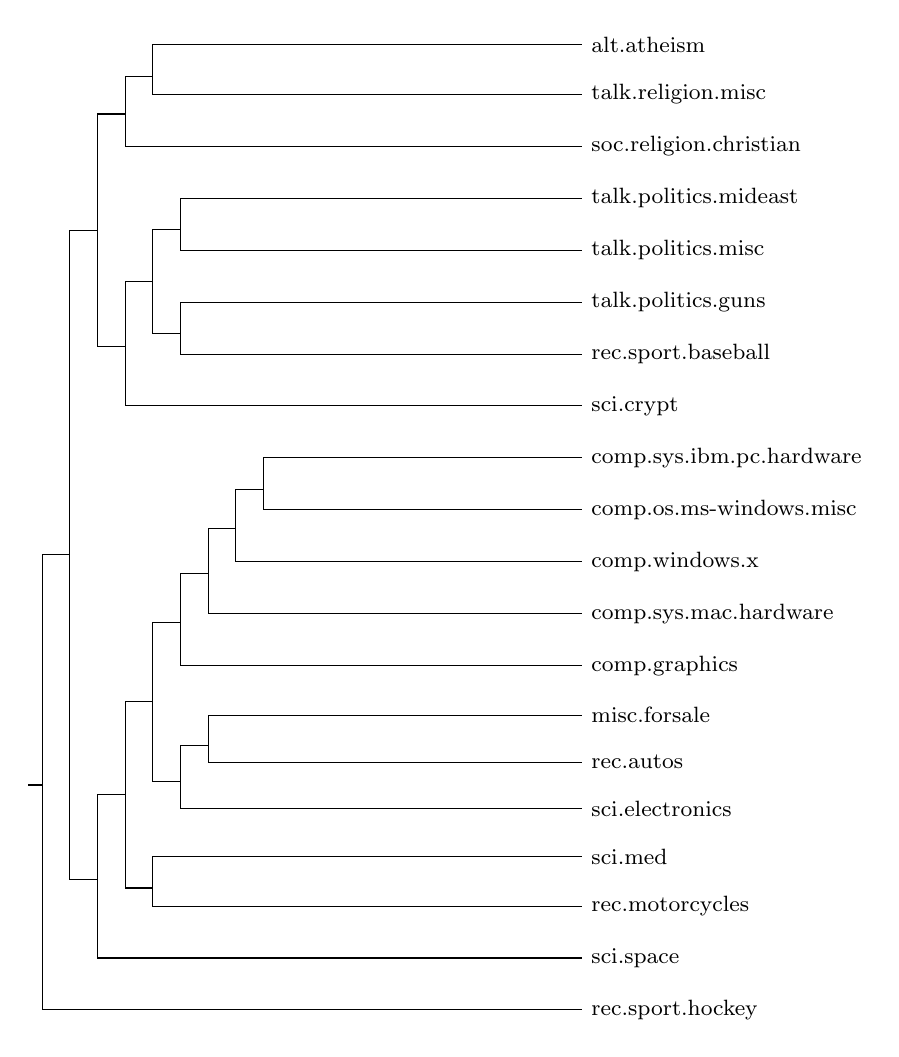
\begin{tikzpicture}
\tikzset{font=\footnotesize}
\tikzset{anchor=base}
\tikzset{sibling distance=5pt}
\tikzset{level distance=10pt}
\tikzset{frontier/.style={distance from root=200}}
\tikzset{grow=right}
\tikzset{every tree node/.style={anchor=base west}}
\tikzset{edge from parent/.style={draw, edge from parent fork right}}
\Tree [ rec.sport.hockey [ [ sci.space [ [ rec.motorcycles sci.med ] [ [ sci.electronics [ rec.autos misc.forsale ] ] [ comp.graphics [ comp.sys.mac.hardware [ comp.windows.x [ comp.os.ms-windows.misc comp.sys.ibm.pc.hardware ] ] ] ] ] ] ] [ [ sci.crypt [ [ rec.sport.baseball talk.politics.guns ] [ talk.politics.misc talk.politics.mideast ] ] ] [ soc.religion.christian [ talk.religion.misc alt.atheism ] ] ] ] ] 

\end{tikzpicture}

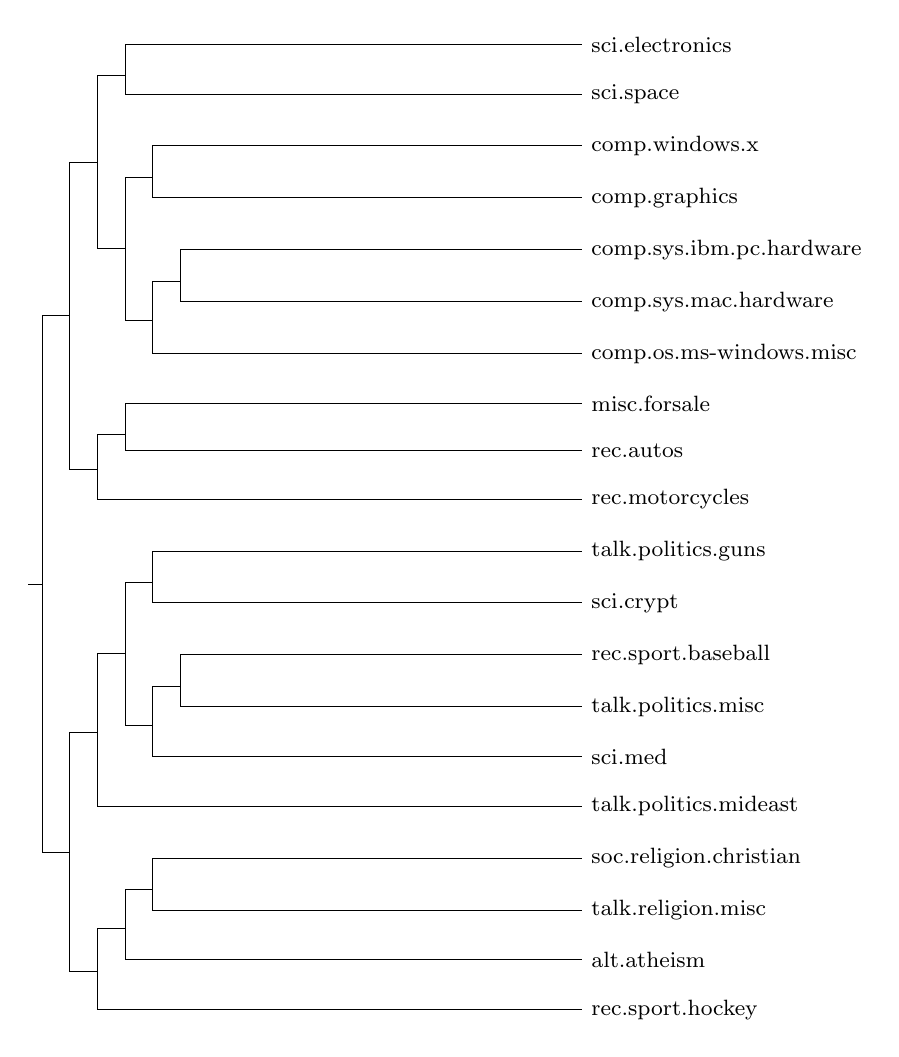
\begin{tikzpicture}
\tikzset{font=\footnotesize}
\tikzset{anchor=base}
\tikzset{sibling distance=5pt}
\tikzset{level distance=10pt}
\tikzset{frontier/.style={distance from root=200}}
\tikzset{grow=right}
\tikzset{every tree node/.style={anchor=base west}}
\tikzset{edge from parent/.style={draw, edge from parent fork right}}
\Tree [ [ [ rec.sport.hockey [ alt.atheism [ talk.religion.misc soc.religion.christian ] ] ] [ talk.politics.mideast [ [ sci.med [ talk.politics.misc rec.sport.baseball ] ] [ sci.crypt talk.politics.guns ] ] ] ] [ [ rec.motorcycles [ rec.autos misc.forsale ] ] [ [ [ comp.os.ms-windows.misc [ comp.sys.mac.hardware comp.sys.ibm.pc.hardware ] ] [ comp.graphics comp.windows.x ] ] [ sci.space sci.electronics ] ] ] ] 

\end{tikzpicture}

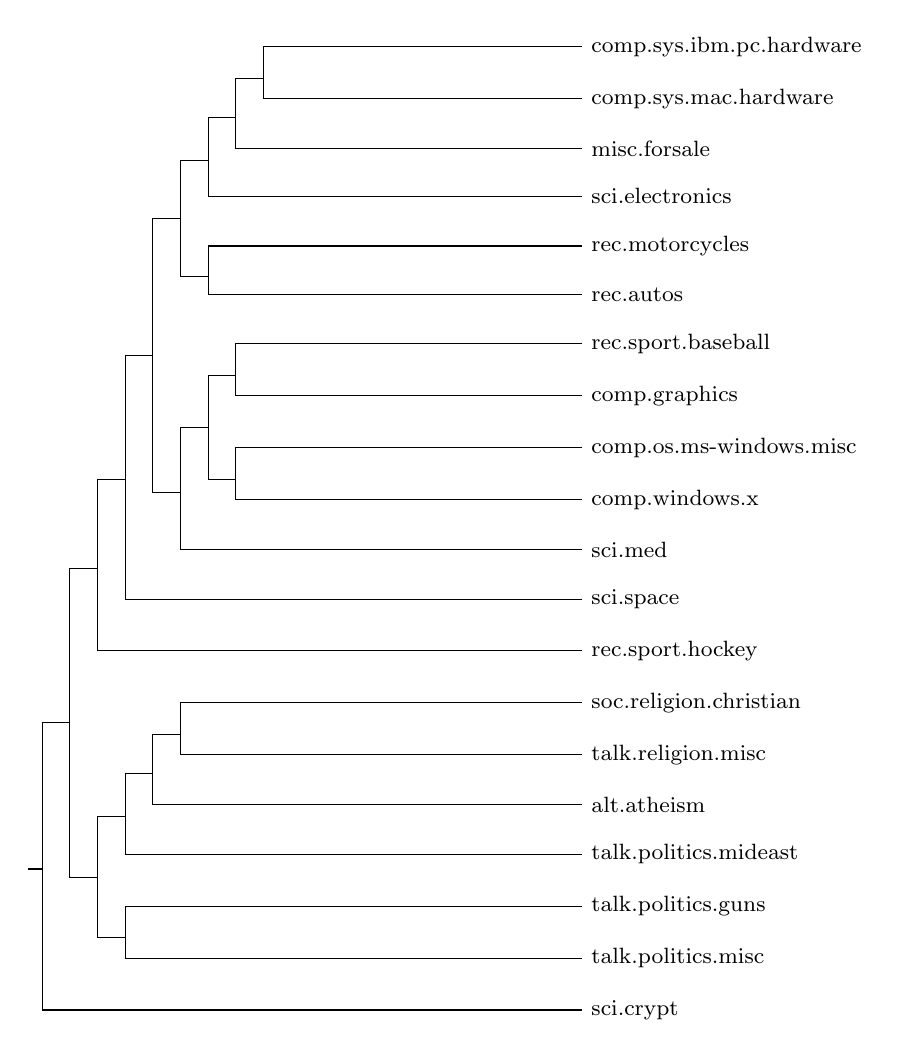
\begin{tikzpicture}
\tikzset{font=\footnotesize}
\tikzset{anchor=base}
\tikzset{sibling distance=5pt}
\tikzset{level distance=10pt}
\tikzset{frontier/.style={distance from root=200}}
\tikzset{grow=right}
\tikzset{every tree node/.style={anchor=base west}}
\tikzset{edge from parent/.style={draw, edge from parent fork right}}
\Tree [ sci.crypt [ [ [ talk.politics.misc talk.politics.guns ] [ talk.politics.mideast [ alt.atheism [ talk.religion.misc soc.religion.christian ] ] ] ] [ rec.sport.hockey [ sci.space [ [ sci.med [ [ comp.windows.x comp.os.ms-windows.misc ] [ comp.graphics rec.sport.baseball ] ] ] [ [ rec.autos rec.motorcycles ] [ sci.electronics [ misc.forsale [ comp.sys.mac.hardware comp.sys.ibm.pc.hardware ] ] ] ] ] ] ] ] ] 
\end{tikzpicture}

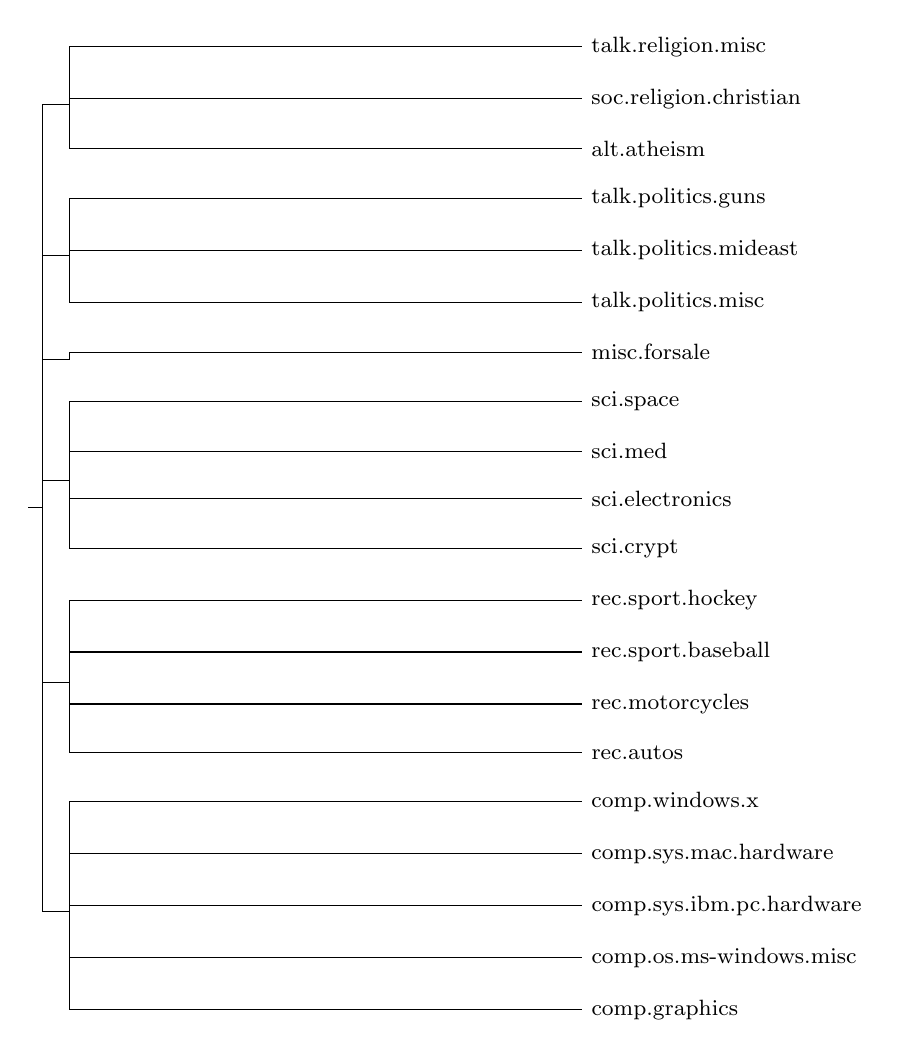
\begin{tikzpicture}
\tikzset{font=\footnotesize}
\tikzset{anchor=base}
\tikzset{sibling distance=5pt}
\tikzset{level distance=10pt}
\tikzset{frontier/.style={distance from root=200}}
\tikzset{grow=right}
\tikzset{every tree node/.style={anchor=base west}}
\tikzset{edge from parent/.style={draw, edge from parent fork right}}
\Tree [ [ comp.graphics comp.os.ms-windows.misc comp.sys.ibm.pc.hardware comp.sys.mac.hardware comp.windows.x ] [ rec.autos rec.motorcycles rec.sport.baseball rec.sport.hockey ] [ sci.crypt sci.electronics sci.med sci.space ] [ misc.forsale ] [ talk.politics.misc talk.politics.mideast talk.politics.guns ] [ alt.atheism soc.religion.christian talk.religion.misc ] ] 
\end{tikzpicture}


\section{Related Work}

\bmcomment{Add footnote about relationship between norm in objective 
and
Mahalanobis norm (just for people in group who look at 
this later)} \nascomment{not sure this is critical}

\bmcomment{Here are some things to possibly write about:}

Self-paced learning \citep{kumar2010self}. \bmcomment{Note relationship
between this and current objective}

Curriculum Learning \citep{bengio2009curriculum}.

Confidence weighted learning \citep{dredze2008confidence}.

Ed Hovy inter-annotator agreement cost \citep{plank2014learning}

Hidden variable learning by state splitting mentioned in 
\url{http://www.cs.cmu.edu/~nasmith/papers/career-proposal-2010.pdf} 
\citep{petrov2011coarse}.

Finite state output encodings mentioned in 
\url{http://www.cs.cmu.edu/~nasmith/papers/career-proposal-2010.pdf}
\citep{loper2008encoding}

\subsection{Future Work and Conclusions}

\bmcomment{Is there anything else that I forgot?}

In future work, richer representations of prediction error types
($\mathcal{S}$) might be pursued.  For example, classes might be 
constructed based on frequencies of classes, with the rarest labels forming
a group.  For structured output spaces such as natural language
parsing, the domain might suggest
groups of errors; post hoc analysis of $\mathbf{e}$ might, in turn,
suggest ways to improve the model through feature
engineering.\footnote{We note an interesting parallel to the
  \emph{ceteris paribus} reasoning suggested by inspection of
linear model weights $\mathbf{w}$; inspecting $\mathbf{e}$ shows,
``all other things equal,'' a scaling of error types by ease-of-avoidance.}
Our framework is easily extended to let these classes depend on
the input or metadata as well, allowing very rich parameterizations of
learnable cost functions.  Recall that these classes need not be mutually exclusive.

Alternative ways to estimate $\mathbf{n}$ might also be considered,
such as using a more sophisticated model to estimate bounds on error
frequencies in the training set.  More generally, characterizations of
ease might be developed through alternate means, such as the
stability measure from learning theory \citep{mukherjee2006learning},
which might offer insight into the generalizability of predictions
involving a particular label.

We concede that our notion of ``ease'' merges several concepts that
might be treated separately.  These include the reliability of the
labels in training data, the distinctiveness of the labels given the
model family (choice of features), the learnability of each label
given the number of instances it has in the training set, and the
overall similarity of the training distribution to the ``true'' one.
We believe it is an open theoretical question how these various
notions might relate to learning guarantees.

\bmcomment{Add recommendation about doing synthetic data experiments
with more features}

\bmcomment{Get rid of ns}

%\subsubsection*{Acknowledgments}

%Use unnumbered third level headings for the acknowledgments. All
%acknowledgments go at the end of the paper. Do not include 
%acknowledgments in the anonymized submission, only in the 
%final paper. 

\bmcomment{The 'references' heading given by the 
bibliography command is the wrong size font.  Needs to
be the size of a 'third level heading'.  How to change this?}
\nascomment{maybe the problem comes from using natbib?}

\bibliography{refs}

\end{document}
